\documentclass[runningheads]{llncs}

\usepackage[T1]{fontenc}
\usepackage{graphicx}
\usepackage{hyperref}
\usepackage{color}
\usepackage{booktabs}
\usepackage{array}
\usepackage{listings}
\usepackage{float}
\usepackage[inline]{enumitem}
\usepackage{tikz}\usetikzlibrary{positioning}
\usepackage{xcolor}
\newcommand{\todo}[1]{\textcolor{red}{\textbf{[TODO: #1]}}}

\renewcommand\UrlFont{\color{blue}\rmfamily}
\usepackage{xcolor}

\begin{document}

\title{LACK: A Knowledge Graph of Agents and Influence Networks in Climate Lobbying}

\author{Enrico Daga\inst{1} \and
Monika Mačiulienė\inst{2} \and
Gregoire Burel\inst{1} \and
Jason Carvalho\inst{1} \and
Arianna Graciotti\inst{3} \and
Harith Alani\inst{1} }

\authorrunning{E. Daga et al.}

\institute{Knowledge Media Institute, The Open University, Milton Keynes, UK \\
\email{\{enrico.daga, jason.carvalho, gregoire.burel, harith.alani\}@open.ac.uk} \and
Kaunas University of Technology, Kaunas, Lithuania \\ \email{monika.maciuliene@ktu.lt} \and University of Groningen, Netherlands\\ \email{a.graciotti@rug.nl}}

\maketitle
% PLACEHOLDER: Resource links block (required by submission format)
% Resource type: Knowledge Graph and Ontology
% License: CC BY 4.0
% DOI: [to be assigned]
% URL: https://climatesense-project.eu/lack/

\begin{abstract}
Organised lobbying against climate action is extensively documented by investigative platforms such as DeSmog and LobbyMap, yet the information they produce remains fragmented, heterogeneous, and difficult to analyse at scale. We present LACK (Lobbying Agents, Climate, and Knowledge), a knowledge graph of ~28k entities and ~200k typed relations — covering affiliations, funding ties, managers, and partnerships — constructed from over 2k web profiles.
To our knowledge, LACK is the first knowledge graph resource dedicated to climate lobbying networks, enabling structured, cross-domain querying of agents, funding relationships, and influence strategies at scale.
We demonstrate its analytical potential through a use case and validate its utility with domain experts from the investigative journalism and climate accountability sector.

\keywords{Knowledge Graph \and Climate Lobbying \and Relation Extraction \and Ontology \and Linked Data \and FAIR Data}
\end{abstract}


% Resource links (required by submission format)
\noindent\textbf{Resource type:} Knowledge Graph\\
\textbf{License:} Creative Commons Attribution 4.0 International (CC BY 4.0)\footnote{
\url{https://creativecommons.org/licenses/by/4.0/}}\\
\textbf{DOI: 10.5281/zenodo.19846036}\\
\textbf{Namespace:} \url{https://purl.net/climatesense/lack/ns#}
\\\textbf{URL:} \url{https://climatesense-project.eu/lack/}

%-----------------------------------------------------------------------

\section{Introduction}
\label{sec:introduction}
Lobbying networks to undermine public trust in climate science and delay effective policy action are extensively documented by investigative journalists and civil society organisations, including dedicated platforms such as DeSmog~\cite{desmog} and InfluenceMap's LobbyMap~\cite{lobbymap}, which publish nearly 2000 profiles of people and organisations who lobby against climate action and policy.
Despite the breadth of such work, the resulting information remains siloed across heterogeneous platforms and is published primarily in long-form prose, organised around organisations rather than around the individuals, roles, and relationships that constitute lobbying networks. 
As a consequence, even basic questions, such as who funds a given think tank, which staff previously worked for fossil fuel companies, or which board members sit across multiple front groups, require tedious manual cross-referencing across sites with incompatible structures. 
Representing this domain as a knowledge graph makes such relational knowledge explicit and queryable at scale.
% Despite the breadth of such work, information remains siloed, heterogeneous
% in format, and difficult to query or analyse computationally at scale.
% This paper presents work carried out within the ClimateSense
% project~\cite{climatesense}, which builds tools to monitor and analyse climate
% misinformation across geospatial, temporal, and topical dimensions.
% Consider an investigative journalist seeking to understand the network behind
% a prominent climate sceptic think tank: who funds it, who sits on its board,
% which staff have previously worked for fossil fuel companies, and whether those
% individuals are linked to other lobbying groups.
% The information needed exists, spread across DeSmog, LobbyMap, and Wikidata, but in incompatible formats, organised around different rationales, and
% not linked, making even this single question require hours of manual cross-referencing.
% The problem is compounded by the temporal dimension: people scatter across
% organisations, funding arrangements may be indirect, and front groups are created
% and dissolved; yet this dynamic structure is difficult to query across sources in an integrated way.

In this paper, we present LACK (Lobbying Agents, Climate, and Knowledge), a knowledge graph of persons and organisations involved in lobbying against climate science and policy, constructed using a composite pipeline combining LLM, web search, and APIs, guided by a purpose-built lightweight ontology.

Specifically, we contribute:
\begin{itemize}
    \item The \textbf{LACK ontology}, a purpose-built OWL vocabulary covering
    the key relation types in the climate lobbying domain.
    \item The \textbf{LACK knowledge graph}, comprising relations between persons and organisations, extracted from more than 2k source documents across two authoritative sources, linked to Wikidata and DBpedia,
    and published as Linked Open Data under a CC BY 4.0 licence.
%    \item An \textbf{LLM-based relation extraction pipeline}, a reusable and    evaluated method for extracting typed, temporally annotated relations from investigative journalism text.
    \item A demonstration of the \textbf{utility of LACK for real-world investigative tasks} in the climate accountability sector, validated through evaluation with domain experts from investigative journalism.
%	\item An \textbf{evaluation with domain experts} from the investigative    journalism and climate accountability sector, assessing the utility and value of the resource for real-world investigative tasks.
%    \item A \textbf{sustainability and maintenance plan}, situating LACK within
%    the ongoing ClimateSense project~\cite{climatesense} and committing to
%    continued updates as source corpora expand.
\end{itemize}

%\paragraph{Paper Structure.}
The remainder of this paper is structured as follows.
Section~\ref{sec:related} situates LACK in the related literature. Section~\ref{sec:extraction} describes the knowledge extraction pipeline, and Section~\ref{sec:ontology} presents the ontology. Section~\ref{sec:construction} covers knowledge graph construction, while Section~\ref{sec:resource} details availability, licensing, and sustainability. Section~\ref{sec:usecase} illustrates case studies, and Section~\ref{sec:evaluation} reports on pipeline evaluation and expert assessment. Section~\ref{sec:conclusion} concludes with directions for future work.
\section{Background and Related Work}
\label{sec:related}

Corporate lobbying has demonstrable consequences for climate policy outcomes.
Brulle~\cite{brulle2018climate} maps US climate-lobbying expenditure across industry sectors, and Meng and Rode~\cite{meng2019social} estimate that lobbying lowered the probability of enacting the Waxman--Markey Cap-and-Trade Bill (a crucial climate action bill in the US) by 13 percentage points, with an estimated welfare loss of roughly \$60 billion.
More recently, Leippold, Sautner and Yu~\cite{leippold2024corporate} document a \emph{camouflaging trend}, whereby firms increasingly conceal climate lobbying behind opaque legislative references, while Baehr, Bare and Heddesheimer~\cite{baehr2026climate} show across more than 11{,}000 firms that earnings-call \emph{climate exposure} systematically predicts whether, how much, and where a firm lobbies.
Understanding lobbying therefore requires more than aggregate spending figures: it requires modelling the underlying network of actors, funders, and affiliations through which climate-policy influence is organised and exerted.

\begin{sloppypar}Investigative platforms partly address the documentation challenge.
DeSmog~\cite{desmog} profiles individuals and organisations involved in denial and lobbying; LobbyMap~\cite{lobbymap} tracks corporate engagement with climate policy; Skeptical Science~\cite{skepticalscience} curates statements attributed to prominent misinformation actors; and Oreskes and Conway~\cite{oreskes2011merchants} analyse strategies used to manufacture doubt about scientific consensus.
These resources are invaluable but heterogeneous, siloed, and not interlinked in any form amenable to computational analysis.
Concurrent efforts such as the UCL \emph{AI-Powered Climate Lobbying Database}~\cite{uclclimatelobbying} reflect the recognised need for better support, automating text extraction and network analysis using large language models.\end{sloppypar}

In the Semantic Web community, CimpleKG~\cite{burel2024cimplekg} provides a continuously updated knowledge graph on misinformation and fact-checks across domains, currently being extended within the ClimateSense project~\cite{climatesense} with climate-specific classifiers, while ClimaFactsKG~\cite{burel2025climafactskg} structures scientific evidence countering climate misinformation; both, however, target claim verification rather than lobbying actor networks.
Knowledge graphs have also been adopted as infrastructure for investigative journalism~\cite{opdahl2022semantic,gallofre2022jkp,berven2020kg,alexander2023manifesto,motta2025epistemology}, but with a focus on news content and event extraction rather than political and corporate actors.
Adjacent Linked Open Data efforts cover political discourse, including the European Parliament debates~\cite{van2016debates} and the digitised Canadian parliamentary record~\cite{beelen2017digitization}, but model what political actors say in formal proceedings rather than the off-stage networks of funding, affiliation, and personnel through which lobbying influence operates.

Constructing such a graph requires entity resolution and entity linking, both well-studied: recent surveys cover end-to-end ER pipelines~\cite{christophides2020er} and neural EL methods~\cite{sevgili2022neural}, with state-of-the-art systems combining candidate retrieval, learned similarity, and graph-aware disambiguation~\cite{ayoola2022refined}.
Large language models have more recently been applied directly to entity matching, often matching or exceeding supervised baselines without task-specific training~\cite{peeters2025llmem}.
LLM-driven approaches fit the climate-lobbying setting: source documents demand contextual disambiguation, and many mentions are long-tail entities absent from general-purpose knowledge bases.
LACK's hybrid pipeline (Section~\ref{sec:extraction}) reflects these constraints, combining knowledge-base candidate retrieval, LLM-based disambiguation, and a web search fallback.

What is missing is a machine-readable representation of the actors and relationships at the core of climate lobbying.
LACK fills this gap as a Wikidata-linked knowledge graph built from investigative sources through an evaluated extraction pipeline and published as Linked Open Data.
\begin{figure}[t]
  \centering
  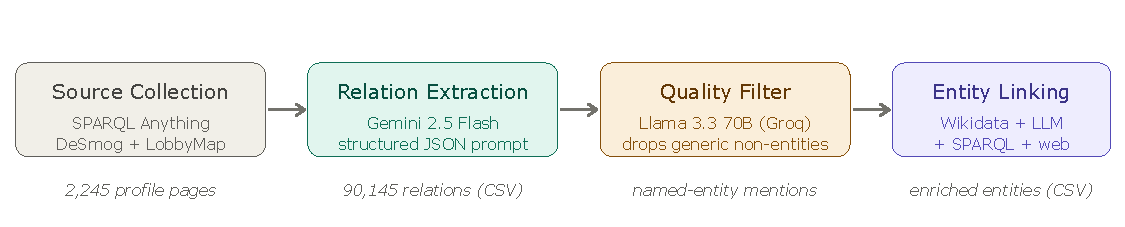
\includegraphics[width=\textwidth]{figures/lack-acquisition-pipeline.pdf}
  \caption{The LACK knowledge acquisition pipeline.
  Each stage is annotated with the model or tool used and the artefact produced.
  The final output feeds into knowledge graph construction (Section~\ref{sec:construction}).}
  \label{fig:acquisition-pipeline}\vspace{-0.3cm}
\end{figure}
\section{Knowledge Acquisition}
\label{sec:extraction}
\paragraph{Requirements and Competency Questions.}
Knowledge requirements were elicited by the authors through informal inductive analysis of ten DeSmog profile pages, manually tagging recurring information types, with emphasis on relations between persons, organisations, and policy actors.
The resulting categories were consolidated into twelve competency questions (CQ1--CQ12) covering four areas (\textit{Transparency and Disclosure}, \textit{Network Structure}, \textit{Temporal Reasoning}, \textit{Identity and Deduplication}), with the resulting ontology subsequently validated for relevance with domain experts (Section~\ref{sec:evaluation}).
The first eleven (CQ1--CQ11) are listed in Table~\ref{tab:coverage} and drove the design of both the ontology (Section~\ref{sec:ontology}) and the extraction pipeline; CQ12, on identity and deduplication, is addressed by the entity linking step described later in this section.
The full text of each question is available on the LACK website\footnote{\url{https://climatesense-project.eu/lack/ontology.html}}.
%
% \paragraph{Sources.}
% LACK was built from the two most comprehensive English-language databases dedicated to climate-lobbying actors\footnote{Pages accessed in December 2025.}; other relevant sources, such as Sceptical Science~\cite{skepticalscience} and SourceWatch, are left to future work.
% \textbf{DeSmog Climate Disinformation Database}~\cite{desmog} is maintained by DeSmog, an international investigative journalism organisation founded in 2006, philanthropically funded, with editorial standards regulated in the UK by IMPRESS, and widely cited by journalists, academics, and policymakers.
% The profile of Cambridge Analytica\footnote{\url{https://www.desmog.com/cambridge-analytica/}}, for example, documents background, fossil fuel connections, funding, key personnel with tenure periods, and a chronological record of notable actions.
% We collected all 943 profile pages listed in the database, typically covering positions on climate science, affiliations, funding sources, and public statements.
% \textbf{LobbyMap}~\cite{lobbymap}, maintained by InfluenceMap (an independent, non-profit think tank founded in 2015), provides analyst-scored assessments of corporate and industry association engagement with climate policy for approximately 1,000 companies and 330 associations, benchmarked against IPCC science.
% The profile of the Business Council of Australia\footnote{\url{https://lobbymap.org/influencer/The-Business-Council-of-Australia}}, for example, provides an overall engagement assessment, a narrative summary of positions across policy areas, a scored evidence matrix by policy query and source, and links to the primary evidence.
% We collected the 964 profile pages from the LobbyMap Scores analysis, plus a further 338 obtained by following links to organisations referenced within them but not themselves in LobbyMap Scores (1,302 pages in total).
% The two sources are complementary: DeSmog focuses on individuals and think tanks involved in active disinformation, while LobbyMap covers corporations and industry associations engaging with policy; well-known actors appear in both.
% The initial set of pages was collected using SPARQL Anything~\cite{daga2021opinionated}, querying the HTML source of the DeSmog Climate Disinformation Database and the JSON feed underlying the LobbyMap Scores leaderboard table.

\paragraph{Sources.}
LACK was built from the two most comprehensive English-language databases dedicated to climate-lobbying actors\footnote{Pages accessed in December 2025.}; other sources, such as Sceptical Science~\cite{skepticalscience} and SourceWatch, are left to future work.
\textbf{DeSmog Climate Disinformation Database}~\cite{desmog}, maintained by DeSmog (an international investigative journalism organisation founded in 2006 and philanthropically funded), profiles individuals and organisations involved in climate denial, typically covering positions on climate science, affiliations, funding sources, and public statements; we collected all 943 profile pages.
\textbf{LobbyMap}~\cite{lobbymap}, maintained by InfluenceMap (an independent non-profit think tank founded in 2015), provides analyst-scored, IPCC-benchmarked assessments of corporate and industry-association engagement with climate policy for approximately 1{,}000 companies and 330 associations; we collected the 964 LobbyMap Scores profiles plus 338 further organisations referenced within them (1,302 pages total).
The two sources are complementary: DeSmog focuses on individuals and think tanks involved in active disinformation, while LobbyMap covers corporations and industry associations engaging with policy; well-known actors appear in both.
The pages were collected using SPARQL Anything~\cite{daga2021opinionated}, querying DeSmog's HTML and the LobbyMap leaderboard JSON feed.

\paragraph{Extraction of relations from web pages.}
Figure~\ref{fig:acquisition-pipeline} summarises the full acquisition pipeline.
The competency questions were translated into a defined set of typed relations between two top-level entity types (Person and Organisation), forming the schema for the extraction pipeline.
Relation extraction was performed by prompting Gemini 2.5 Flash~\cite{gemini25}, chosen for its native URL-context tool (which fetches DeSmog pages directly, avoiding bespoke scraping) and the team's available access.
The prompt specifies the allowed relation types with their definitions, a strict JSON output schema (\texttt{Relation} objects with source, target, type, optional \texttt{xsd:gYear} temporal annotations, a description, and evidence URLs), and a constraint to use only the provided page as evidence.
For DeSmog, page content was fetched directly by the model via Gemini's native URL context tool.
For LobbyMap, HTML pages were fetched separately and passed as input to the model.
The pipeline iterates over all collected profile URLs, invoking the model once per page and storing output as one JSON file per profile, with resumption logic to skip already-processed pages.
After each run, a validation routine identified and deleted malformed or empty outputs; the extraction was then re-run on failed pages, repeating until all pages were successfully processed.
The process, implemented in a Google Colab notebook (deposited~\cite{lack-re}), outputs a CSV file for each data source with a row for each relation, with columns for source, target, their types, relation type, temporal annotations, a natural-language description, and the evidence URL.

\paragraph{Entity Linking.}
The relation extraction step produces entities as surface form strings rather than authoritative identifiers, requiring three further operations: deduplication, entity resolution, and linking to Wikidata~\cite{wikidata}, with Wikipedia as a secondary target or, where no knowledge base entry exists, identification via a dedicated public web page.
The input to this step is a pair of (entity name, evidence link) — the surface form and the source profile page where it appeared — augmented by natural language context sentences aggregated from the previous step.
The same surface form on the same page is treated as a single entity; the same surface form across different pages is not assumed to refer to the same entity.
%A preliminary quality step filters out generic non-entities using Groq-hosted Llama 3.3 70B~\cite{llama33}.
A preliminary quality step filters out generic non-entities using Groq-hosted Llama 3.3 70B~\cite{llama33}, selected for production cost-efficiency at scale.
An LLM classifier distinguishes concrete named entities from purely descriptive or quantitative strings, flagging expressions such as \texttt{"14 lobbyists"}, \texttt{"200 civil society groups"}, or \texttt{"Gas lobby"} for removal, while retaining named events, initiatives, and borderline collectives that carry a proper name.
For the remaining entities, we apply a hybrid linking pipeline combining Wikidata API candidate retrieval, LLM-based disambiguation, and SPARQL-based verification, with a web search fallback for entities absent from Wikidata.
The pipeline was prototyped using Claude Sonnet 4.6~\cite{claudesonnet46}, chosen for stronger reasoning during design, and executed at scale on Llama 3.3 70B~\cite{llama33} (already justified above) for production cost-efficiency; a larger model may have improved recall on long-tail entities, and we leave this comparison to future work.
% For the remaining entities, we apply a hybrid linking pipeline co-designed with Claude~\cite{claude}, combining Wikidata API candidate retrieval, LLM-based disambiguation, and SPARQL-based verification, with a web search fallback for entities absent from Wikidata.
% The pipeline was designed and prototyped using Claude Sonnet 4.6~\cite{claudesonnet46} and executed at scale using Groq-hosted Llama 3.3 70B~\cite{llama33} for cost efficiency.
Candidate Wikidata entries are retrieved via the Wikidata API, with a Wikipedia search API fallback for entities not indexed there, resolving article titles to Wikidata QIDs.
When a Wikipedia page is found, we produce DBpedia resource links.
Because the \texttt{organisation} type in our data spans a wide range of entity classes — companies, think tanks, PACs, government agencies, events, journals, and coalitions — type-based filtering in Wikidata is unreliable; entity subtype is instead inferred by the LLM from context.
Candidates are passed to the LLM, which selects the best matching QID or returns null, also detecting when a candidate represents a broader parent entity rather than the specific entity itself.
Selected QIDs are verified via SPARQL, retrieving canonical label, Wikipedia sitelink, and parent organisation (via \texttt{P749}/\texttt{P361}).
For entities with no Wikidata match, a web fallback first evaluates the evidence link as a potential primary identifier, then issues an LLM-generated search query via the Google Custom Search API~\cite{googlecse}, with a primary-subject check confirming whether each result page is dedicated to the entity.
The output is an enriched CSV of entities, containing Wikidata URIs, Wikipedia URLs, parent entity links, web page fallbacks, and confidence scores. All code and data are published~\cite{lack-el}.

\paragraph{Evaluation of the extraction output.}
We now evaluate the extracted data: source coverage, the accuracy of extracted relations and entity links, and known limitations.

Our collection covers the DeSmog Climate Disinformation Database and the LobbyMap Scores leaderboard in their entirety as of the time of collection, providing complete coverage with respect to these two curated entry points.
With respect to LobbyMap, the Scores leaderboard covers approximately 1,000 companies and 330 industry associations, but InfluenceMap hosts a broader set of content — including sector-level reports, country profiles, and policy engagement assessments — that was not included in the current collection.
Extending coverage to these additional sources remains a direction for future work.

Relation extraction was evaluated on a sample of 300 relations drawn from 8 randomly selected DeSmog profile pages.
Three annotators (the authors) worked in pairs, each pair covering approximately 100 relations, with disagreements resolved by discussion.
Each relation was assessed on three dimensions: truthfulness (is the relation supported by the source page?), validity (is the relation type and its domain and range correctly applied according to the schema?), and temporal correctness (are the temporal annotations accurate?)\footnote{Full annotation guidelines: \url{https://bit.ly/lack_42bhqzl}.}.
Truthfulness accuracy is 0.93 (0.99 with partial credit), validity 0.907 (0.95 with partial), and temporal correctness 0.797 (0.91 with partial), where partial credit captures approximately correct extractions.
The main source of partly correct answers relates to the conflation of specific sub-roles with the coarser schema relations: the model frequently uses \texttt{is president of} or \texttt{is director of} where the source text indicates a more specific role such as vice-president, deputy director, or departmental director.
A recurrent validity issue is the misapplication of organisation-level relations to person-organisation pairs: for example, \texttt{has partner} was used when a person holds a partner title at a law or consulting firm, whereas the relation was intended to connect two organisations in a formal partnership.
Temporal correctness is the least accurate dimension, with errors arising from missing dates, incorrect inference of date ranges, and ambiguity in encoding point-in-time vs.\ interval information, but still reaching ~0.80\% of accuracy.

Entity linking was evaluated on 225 entities from the same pages as the previous evaluation, against a curated gold standard\footnote{Gold standard preparation: \url{https://bit.ly/lack_3QQPRsD}} produced by four annotators (the authors), each covering approximately 56 entities, with a subset supervised by a second annotator and disagreements resolved by discussion.
Each entity was assessed on five dimensions: entity subtype correctness, Wikidata URI, Wikipedia URL, parent entity, web page (where applicable); see-also links were assessed separately.
Accuracy is high across most dimensions, with see-also at 0.96, parent entity at 0.94, Wikidata URI and Wikipedia URL at 0.88, entity subtype at 0.86, and web page at 0.84, indicating that the pipeline reliably identifies and links entities across all primary output fields.
For the two fields whose gold reference can be precisely defined---Wikidata URI and Wikipedia URL---precision and recall are also balanced (0.93/0.85 and 0.88/0.88 respectively), confirming that the pipeline neither over- nor under-produces links for these dimensions.
The weakest dimension in terms of precision is web page (0.49 precision, 0.59 recall), reflecting the difficulty of identifying a single canonical web presence.
Parent entity, despite high overall accuracy, exhibits the most informative error pattern (precision 0.79, recall 0.73): the dominant failure mode is over-eager parent assignment for foundations, transition teams, and political campaigns where no real parent organisation exists in Wikidata, alongside a smaller number of cases in which a meaningful parent was missed entirely.
Of the 219 entities with see-also content in the gold standard, only 19 included at least one novel URL beyond the evidence link, contributing 44 additional reference pages in total ($\approx 8.4\%$).

Of the 27,945 entities in the KG, 10,189 (36.5\%) are linked to Wikidata or DBpedia, while 17,756 (63.5\%) remain without an external identifier --- a proportion that is consistent across both sources: 64.4\% of DeSmog-only entities and 65.7\% of LobbyMap-only entities are NIL.
This high NIL rate is not a pipeline failure but a domain characteristic: the climate lobbying ecosystem is densely populated with minor think tank staff, obscure industry consultants, short-lived coalitions, and regional trade bodies that are simply not represented in general-purpose knowledge bases such as Wikidata.
By contrast, entities appearing in both sources --- those prominent enough to be independently documented by DeSmog and LobbyMap --- are linked at a rate of 95.7\% (488 out of 510), confirming that the pipeline reliably identifies well-known actors.
NIL entities will be resolvable within the KG via their LACK URI and retain their label and source provenance; web page and parent entity fields, included as \textit{see also} statements, captured during entity linking but not yet promoted to \texttt{owl:sameAs} assertions, offer a path to further grounding and are left to future work.
A residual data quality issue --- 29 entities with inconsistent type assignments across pages --- will be resolved in a future release.


\section{The LACK Ontology}
\label{sec:ontology}

\paragraph{Ontology Engineering Methodology.}
The LACK ontology was designed following a bottom-up, requirements-driven process.
The starting point was an analysis of the knowledge needs raised by the investigative sources --- what types of relationships are expressed in DeSmog and LobbyMap profiles? --- which were formalised as a set of competency questions (CQ1--CQ12, see Section~\ref{sec:resource} and the LACK website\footnote{\url{https://climatesense-project.eu/lack/ontology.html}}).
These competency questions drove the design of the knowledge extraction pipeline described in Section~\ref{sec:extraction}, and were subsequently refined based on data quality assessment carried out at the end of the extraction process.
A guiding design principle throughout was to represent only what could be reliably and automatically produced by the extraction pipeline, deliberately excluding relation types that could not be extracted with sufficient confidence.
This constraint was essential to maximise the quality of a resource that cannot be fully verified manually and is intended to scale to very large volumes of data.

\paragraph{Motivation for a New Vocabulary.}
Two main considerations motivated the development of a new vocabulary rather than reusing an existing one.
First, existing general-purpose vocabularies such as schema.org do not adequately cover the domain-specific relationships present in climate lobbying data: the schema.org alignment exercise revealed systematic inverse direction mismatches and an absence of equivalents for lobbying-specific relations such as \emph{lobbied for}, \emph{conducted public relations for}, or \emph{incorporated}~\cite{schemaorg}.
Second, a key analytical goal of LACK is to support graph-based network analysis --- centrality, community detection, shortest path --- which requires direct typed links between entity nodes.
Schema.org's recommended pattern for named organisational roles (wrapping relations in materialised \texttt{schema:Role} intermediary nodes) would fragment the graph and complicate traversal, making it unsuitable for this purpose.

\paragraph{Top-Level Types.}
The ontology defines two top-level classes: \texttt{lack:Person}, representing an individual human being, and \texttt{lack:Collective}, representing any group of people organised around a shared purpose.
The choice of \texttt{Collective} over the more intuitive \texttt{Organisation} was motivated by quality analysis during extraction: the data revealed that many entities appearing in the sources were not organisations in the strict sense, but events (conferences, summits), journals, campaigns, committees, and networks.
Introducing \texttt{Collective} as a deliberately broad type accommodates this diversity without requiring the extraction pipeline to distinguish between multiple disjoint subclasses --- a distinction it could not make reliably.

\paragraph{Relation Types.}
Table~\ref{tab:ontology} provides a summary of the relation types defined in the ontology, grouped by category, and Figure~\ref{fig:ontology} shows the corresponding schema diagram.
Each relation is defined with a domain, a range, an inverse property, and where applicable a sub-property link within the hierarchy rooted at \texttt{lack:associatedWith} --- the top-level symmetric catch-all relation used when no more specific type applies.
The full vocabulary, including formal definitions and SPARQL examples for each competency question, is available on the LACK website\footnote{\url{https://climatesense-project.eu/lack/ontology.html}}.

\begin{figure}[th]
    \centering
    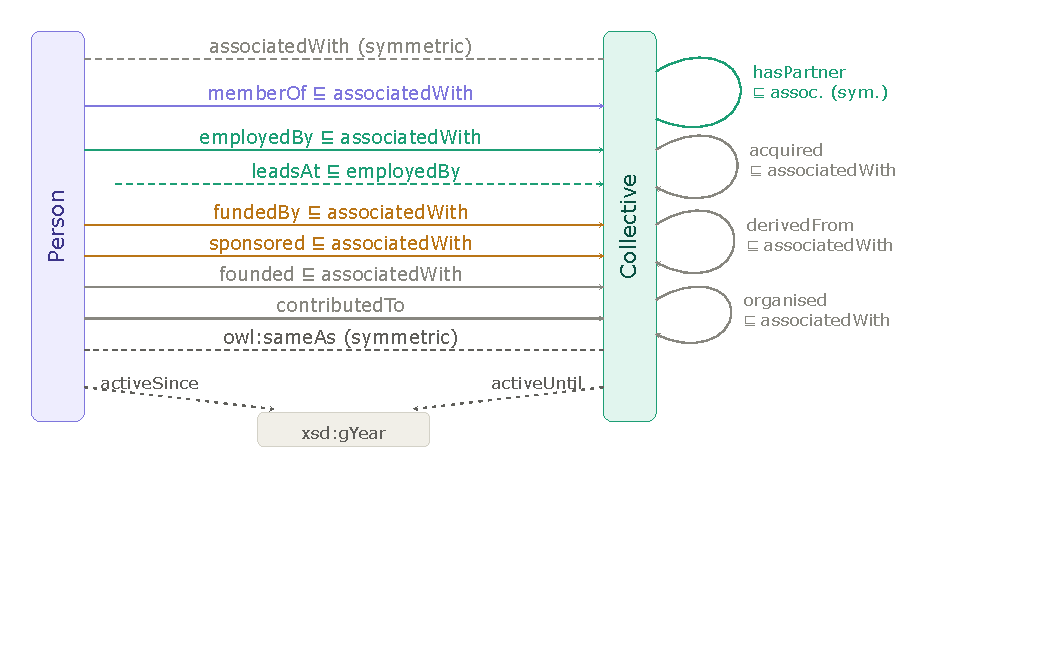
\includegraphics[width=\textwidth]{figures/lack-ontology-diagram.pdf}
    \caption{Schema diagram of the LACK ontology.}
    \label{fig:ontology}
\end{figure}

\begin{table}[t]
\caption{Summary of LACK relation types.}
\label{tab:ontology}
\centering
\small
\begin{tabular}{llllll}
\hline
\textbf{Group} & \textbf{Term} & \textbf{Domain} & \textbf{Range} & \textbf{Inverse} & \textbf{Sub-property of} \\
\hline
Membership   & \texttt{memberOf}      & Person      & Collective  & \texttt{hasMember}       & \texttt{associatedWith} \\
Employment   & \texttt{employedBy}    & Person      & Collective  & \texttt{hasEmployee}     & \texttt{associatedWith} \\
Leadership   & \texttt{leadsAt}       & Person      & Collective  & \texttt{hasLeader}       & \texttt{employedBy} \\
Funding      & \texttt{fundedBy}      & P $|$ C     & P $|$ C     & \texttt{hasFunder}       & \texttt{associatedWith} \\
Sponsorship  & \texttt{sponsored}     & P $|$ C     & P $|$ C     & \texttt{wasSponsoredBy}  & \texttt{associatedWith} \\
Founding     & \texttt{founded}       & P $|$ C     & Collective  & \texttt{wasFoundedBy}    & \texttt{associatedWith} \\
Contribution & \texttt{contributedTo} & P $|$ C     & Collective  & \texttt{hasContributor}  & --- \\
Partnership  & \texttt{hasPartner}    & Collective  & Collective  & (symmetric)              & \texttt{associatedWith} \\
Acquisition  & \texttt{acquired}      & Collective  & Collective  & \texttt{wasAcquiredBy}   & \texttt{associatedWith} \\
Derivation   & \texttt{derivedFrom}   & Collective  & Collective  & \texttt{hasDerivation}   & \texttt{associatedWith} \\
Association  & \texttt{associatedWith}& P $|$ C     & P $|$ C     & (symmetric)              & --- \\
Identity     & \texttt{owl:sameAs}    & P $|$ C     & P $|$ C     & (symmetric)              & --- \\
\hline
\end{tabular}
\end{table}

\noindent All \texttt{lack:} prefixes are omitted from the Term column for brevity. P = \texttt{lack:Person}, C = \texttt{lack:Collective}.

\paragraph{Reuse of External Vocabularies.}
Where established terms are available, the ontology reuses them rather than introducing new ones.
\texttt{owl:sameAs} is used to assert identity between entities --- covering renaming, aliases, and doing-business-as relations.
Provenance is represented using PROV-O~\cite{provo}: each reified statement is linked to a shared \texttt{prov:Activity} (the LACK extraction activity) and a \texttt{prov:SoftwareAgent} (the extraction pipeline), via \texttt{prov:wasGeneratedBy}.
Source attribution is recorded using Dublin Core Terms~\cite{dcterms} (\texttt{dct:source}), pointing to the URL of the source web page from which the relation was extracted.

\paragraph{Temporal Representation.}
Many relationships in the climate lobbying domain are time-bounded: a person leads an organisation for a period, funding flows during a specific interval, or a front group is active only around a key legislative event.
LACK captures this through two mechanisms.
Entity-level temporal bounds are recorded directly on \texttt{lack:Person} and \texttt{lack:Collective} instances using the datatype properties \texttt{lack:activeSince} and \texttt{lack:activeUntil} (range: \texttt{xsd:gYear}).
Relation-level temporal annotations are represented using RDF reification~\cite{rdfprimer}: each temporally annotated triple is reified as an \texttt{rdf:Statement} instance, to which \texttt{lack:since} and \texttt{lack:until} datatype properties are attached.
When a source annotation indicates a point in time rather than an interval (\emph{when}), both \texttt{lack:since} and \texttt{lack:until} are set to the same year value.
RDF reification was chosen over more recent alternatives such as RDF-star, named graphs, and singleton properties in order to ensure broad compatibility with current RDF databases and applications.
Figure~\ref{fig:reification} illustrates this pattern with a concrete example.

\begin{figure}[th]
    \centering
    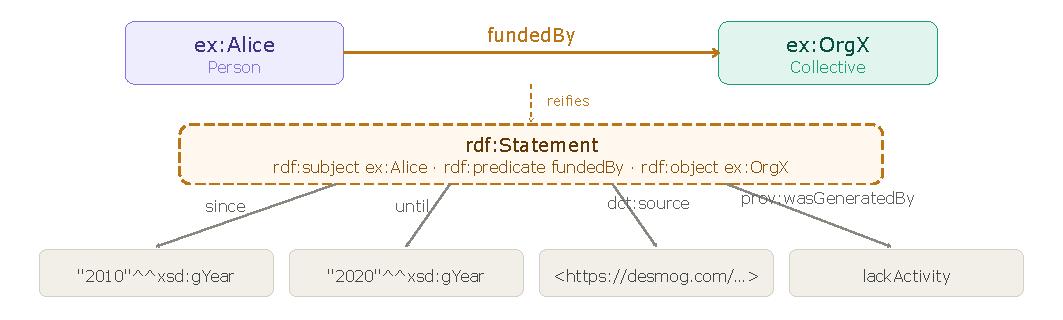
\includegraphics[width=\textwidth]{figures/lack-reification-diagram.pdf}
    \caption{RDF reification of a binary relation, decorated with temporal annotations (\texttt{since}, \texttt{until}), evidence source (\texttt{dct:source}), and provenance (\texttt{prov:wasGeneratedBy}).}
    \label{fig:reification}
\end{figure}

\paragraph{Availability.}
The LACK ontology is identified by the namespace URI \url{https://purl.net/climatesense/lack/ns#} and is available for download in Turtle and OWL Manchester Syntax formats.
It is published under a Creative Commons Attribution 4.0 International (CC BY 4.0) licence.

\section{Knowledge Graph Construction}
\label{sec:construction}

The LACK knowledge graph is produced by a four-phase pipeline that transforms the relation extraction outputs described in Section~\ref{sec:extraction} into a fully materialised, ontology-aligned RDF graph.
Each phase is implemented as a SPARQL or SPARQL-Anything~\cite{sparqlanything} query, executed with the \texttt{fx} command-line tool, making the entire pipeline reproducible from the raw CSV inputs.

\subsection{Phase 1: Relation Alignment}
\label{sec:construction:alignment}

The relation extraction pipeline produces relations expressed as natural-language surface forms (e.g.\ \emph{is a member of}, \emph{has funded}).
The first phase enumerates the distinct relation types appearing across both the Desmog and LobbyMap extraction outputs --- 152 types in total, covering 78,734 relation instances --- and aligns them manually to LACK ontology properties.
The result is a mapping table that associates each surface-form relation type with a canonical ontology IRI (e.g.\ \texttt{lack:memberOf}, \texttt{lack:fundedBy}), which is consumed by all subsequent phases.
This manual alignment step is where domain judgment is applied: surface forms that are ambiguous, too infrequent, or not reliably mappable to any ontology property are flagged and excluded from the graph.

\subsection{Phase 2: Entity URI Generation}
\label{sec:construction:entities}

Stable, dereferenceable IRIs are minted for each entity using a priority scheme over available external identifiers:

\begin{enumerate}
    \item Wikidata QID
    \item Wikipedia page URL
    \item Web page URL
    \item Surface form + evidence link (fallback)
\end{enumerate}

\noindent Each entity IRI takes the form \texttt{lack-entity:\textit{SHA1}}, where the hash is computed from the highest-priority identifier available for that entity.
This scheme ensures that entities with a known Wikidata entry receive a stable, semantically grounded IRI regardless of how they are named in the source data, while still providing a consistent IRI for entities that have no external presence.
Each entity is assigned a top-level type (\texttt{lack:Person} or \texttt{lack:Collective}), a granular subtype (e.g.\ \texttt{lack-type:think\_tank}, \texttt{lack-type:company}), an \texttt{rdfs:label}, and where available an \texttt{owl:sameAs} link to the corresponding Wikidata entity.

\subsection{Phase 3: Relation Graph Construction}
\label{sec:construction:relations}

With entity IRIs in place, the relation triples are constructed from the raw extraction outputs and the relation alignment mappings produced in Phase~1.
A na\"ive join of all inputs would exceed memory constraints, so the phase is split into two steps: first, an entity index is built in memory (mapping surface-form + evidence-link pairs to entity IRIs); second, the index is used to rewrite each extracted relation as a triple using the appropriate LACK ontology property.

Each relation is represented following the pattern established in the ontology (Section~\ref{sec:ontology}): a direct typed triple connects source and target entities, while a reified \texttt{rdf:Statement} carries the evidence URL (\texttt{dct:source}) and, where available, temporal bounds (\texttt{lack:since}, \texttt{lack:until}).
The same logical relation may be attested by multiple evidence sources, yielding multiple reified instances for a single direct triple; the final graph contains 65,527 distinct relation triples and 77,168 reified instances.

\subsection{Phase 4: Provenance}
\label{sec:construction:provenance}

A dedicated provenance query enriches each reified statement with PROV-O~\cite{provo} annotations.
Each statement is linked to a shared \texttt{prov:Activity} representing the LACK extraction activity, and to a \texttt{prov:Agent} identifying the extraction pipeline, via \texttt{prov:wasGeneratedBy}. \texttt{prov:used} arcs collect all source web pages used in any \texttt{rdf:Statement} produced so far.
%This step is kept separate from Phase~3 to maintain a clean separation between the structural construction of the graph and the attachment of process-level metadata.

\subsection{Phase 5: OWL Inference Materialisation}
\label{sec:construction:inference}

Rather than relying on a full OWL reasoner at query time, we materialise the entailments of its ontology as explicit triples using a sequence of SPARQL CONSTRUCT queries.
%This ensures that all queries over the graph are complete with respect to the ontology's axioms without requiring inference-capable infrastructure.
%The materialisation pipeline proceeds in three steps.
First, inverse property pairs are materialised (e.g.\ \texttt{memberOf} / \texttt{hasMember}, \texttt{fundedBy} / \texttt{hasFunder}) for all ten inverse pairs defined in the ontology.
Second, sub-property entailments are propagated: \texttt{leadsAt} triples are promoted to \texttt{employedBy} triples (and correspondingly for their inverses), and all direct sub-properties of \texttt{associatedWith} generate \texttt{associatedWith} triples.
Third, symmetry is closed for \texttt{associatedWith} and \texttt{hasPartner}.
The steps are executed in this order so that triples generated in earlier steps are available as input to later ones, ensuring completeness of the inference closure.
After materialisation, the graph grows from approximately 66,000 relation triples to over 264,000.
\section{Resource Description}
\label{sec:resource}

\vspace{-0.3cm}\section{Use Cases}
\label{sec:usecase}
We demonstrate the value of LACK with two use cases. 
The first use case identifies entities that may be difficult to trace their connection without integrating the data sources\footnote{We present more of these examples on our website: \url{https://climatesense-project.eu/lack/case-studies.html}.}
The second use case cross matches LACK Collectives with the attendees the attendees
most connected LACK Collectives with the attendance list of COP30 (the United Nations Climate Change Conference), and identifies potential investigations.
\begin{sloppypar}
\paragraph{Case study: LACK enables integration of multiple independent sources.} 
We provide two examples with the same structure: two statements, each drawn from a different source — the DeSmog Climate Disinformation Database and LobbyMap — share a common entity that acts as a bridge. 
Neither source mentions the entities cited in the other — yet their combination, through the shared bridge entity, reveals a relationship that no single source makes visible\footnote{The connections revealed are structural, derived from publicly available data; they do not imply wrongdoing, shared intent, or direct collaboration, and are presented as research leads rather than evidential claims.}.

\textit{Example 1: Darren Woods $\rightarrow$ Exxon $\rightarrow$ Heartland Institute}
\noindent\textbf{Bridge entity:} Exxon. \textbf{(InfluenceMap)} Darren Woods \texttt{lack:leadsAt} Exxon; \textbf{(DeSmog)} Exxon \texttt{lack:sponsored} Heartland Institute.
InfluenceMap documents Woods leading Exxon; DeSmog records Exxon as a sponsor of the Heartland Institute, a think tank prominently associated with climate science denial.
Neither source references the other's entity, yet LACK makes the chain explicit, linking a named corporate officer to a climate change denial organisation through his employer --- a pattern generalised by joining \texttt{lack:leadsAt} with \texttt{lack:sponsored} in a single SPARQL query.

\textit{Example 2: Cambridge Analytica $\rightarrow$ BP $\rightarrow$ Business Council of Australia}
\noindent\textbf{Bridge entity:} BP. \textbf{(DeSmog)} Cambridge Analytica \texttt{lack:hasPartner} BP; \textbf{(InfluenceMap)} BP \texttt{lack:memberOf} Business Council of Australia.
DeSmog records a partnership between the data and political consultancy firm Cambridge Analytica and BP, while InfluenceMap separately documents BP's membership of the Business Council of Australia, an industry body with a record of opposing climate legislation.
The two facts originate from different investigative contexts --- political data operations vs.\ fossil fuel industry lobbying in Australia --- and share only BP, yet LACK surfaces this cross-domain, cross-jurisdictional structural connection that neither source exposes alone.
\end{sloppypar}

Tracing such chains allows researchers to surface accountability relationships that are structurally present in the data but invisible within any single source.

% %-----------------------------------------------------------------------
% \subsection*{Case 3: Nick Stavropoulos $\rightarrow$ PG\&E $\rightarrow$ ZETA}

% \noindent\textbf{Source A (DeSmog):} Nick Stavropoulos \texttt{lack:leadsAt} PG\&E.\\
% \textbf{Source B (LobbyMap):} PG\&E \texttt{lack:memberOf} Zero Emission Transportation Association (ZETA).\\
% \textbf{Bridge entity:} PG\&E.

% \smallskip
% \noindent DeSmog profiles Nick Stavropoulos as an executive at PG\&E, the Californian utility. LobbyMap independently records PG\&E's membership of the Zero Emission Transportation Association, an electric vehicle industry coalition. Unlike the preceding cases, the target organisation here is not associated with climate denial; ZETA actively advocates for EV adoption. This case illustrates that LACK captures the full complexity of influence networks — including actors whose affiliations span both fossil fuel infrastructure and clean energy advocacy — rather than mapping only clear-cut disinformation actors.
% \paragraph{LACK as a selective filter on COP30 attendance.}
% Crossing LACK with the COP30 participant list shows that the resource functions as a curated filter on the climate-policy field rather than as a comprehensive registry of attendees. Of 47{,}308 registered delegates and 19{,}298 distinct organisations, 0.11\% and 2.87\% respectively are present in LACK, concentrated in the corporate, financial, and lobby-aligned segments LACK is designed to track. The match rate varies fivefold across UNFCCC participation categories---from 2.2\% for government bodies to 10.2\% for the Global Climate Action cluster---and across national delegations, from 8.1\% for Australia and 6.5\% for France to 0\% for several small states. This unevenness reflects LACK's design (corporate-focused, anglophone, Western-centric) and makes the COP30 cross-reference a useful external probe of the resource's effective scope. 
% %Presence in LACK identifies an attendee as a member of the broader climate-policy field; absence carries no such inference.
\begin{sloppypar}
\paragraph{Case study: LACK's prominent collectives at COP30.}
We cross-referenced LACK's 1{,}000 most heavily-described \texttt{lack:Collective} entities (ranked by outgoing IRI links) with the COP30 participant list via a simple heuristic label match.
Of 944 distinct delegate matches, roughly 70\% flow through observer accreditation channels, 18\% appear in high-income national delegations (EU institutions, BNP Paribas, METI, the World Economic Forum), and only 43 in lower- or low-income country delegations.
A qualitative look at the top-20 scope shows the LACK's most densely connected entities: the US climate countermovement (Heartland, Cato, ALEC, Heritage, Manhattan Institute) --- of which only three (US Chamber of Commerce, Shell, ExxonMobil) appear at COP30 at all.
The cross-reference surfaces two findings worth investigation, which were invisible to either resource alone: the US climate countermovement does not engage with the UNFCCC track, and observer accreditation rather than national delegation is the dominant channel through which LACK-tracked organisations participate in COP.
This is one example of the broader family of analyses LACK enables when paired with any external source of named climate-policy agents. 
\end{sloppypar}

\section{Evaluation}
\label{sec:evaluation}
In this section, we evaluate the LACK KG against two dimensions: coverage with respect to the competency questions and utility of the resource, through a questionnaire with domain experts.

\subsection{Resource Coverage}

\paragraph{Rationale} Resource coverage is evaluated by assessing the extent to which the knowledge graph can answer the competency questions used to drive its design. For each competency question, we identify the ontology relation(s) required to answer it, count the number of triples available for those relations in the KG before and after inferencing, and derive a qualitative coverage estimate. This allows us to assess both the intrinsic density of the extracted data and the contribution of OWL inferencing to query answerability.

%\subsubsection{Research Questions and Competency Questions}

\paragraph{Questions}Table~\ref{tab:coverage} maps each research question to its competency question(s), the ontology relation(s) required to answer it, and the corresponding coverage statistics.



%\subsubsection{Methodology}

\begin{sloppypar}\paragraph{Methodology} For each competency question, we report the number of triples for the relevant relation(s) before and after inferencing, as derived from the KG statistics. We also report the number of distinct entities affected, obtained by running SPARQL queries against the ClimateSense endpoint (\url{https://sparql.climatesense.kmi.tools/climatesense}, graph \texttt{<https://purl.net/climatesense/lack>}). Coverage is classified into three tiers: \textbf{Strong} (more than 5,000 triples), \textbf{Moderate} (between 1,000 and 5,000 triples), and \textbf{Weak} (fewer than 1,000 triples). For competency questions involving temporal annotation (CQ10, CQ11), coverage depends on the proportion of entities and relations decorated with \texttt{lack:activeSince} / \texttt{lack:activeUntil} or with \texttt{lack:since}/\texttt{lack:until} on reified statements; these figures are obtained via dedicated SPARQL queries.\end{sloppypar}

% All queries are run against:
% \begin{itemize}
%   \item Endpoint: \url{https://sparql.climatesense.kmi.tools/climatesense}
%   \item Graph: \texttt{<https://purl.net/climatesense/lack>}
% \end{itemize}
%
% \paragraph{CQ2 --- Funding}
% \begin{lstlisting}[language=SPARQL]
% SELECT (COUNT(DISTINCT ?e) AS ?entities)
% FROM <https://purl.net/climatesense/lack>
% WHERE { { ?e <https://purl.net/climatesense/lack/ns#fundedBy> ?o }
%         UNION
%         { ?s <https://purl.net/climatesense/lack/ns#fundedBy> ?e } }
% \end{lstlisting}
%
% \paragraph{CQ3 --- Membership}
% \begin{lstlisting}[language=SPARQL]
% SELECT (COUNT(DISTINCT ?e) AS ?entities)
% FROM <https://purl.net/climatesense/lack>
% WHERE { { ?e <https://purl.net/climatesense/lack/ns#memberOf> ?o }
%         UNION
%         { ?s <https://purl.net/climatesense/lack/ns#memberOf> ?e } }
% \end{lstlisting}
%
% \paragraph{CQ4 --- Leadership}
% \begin{lstlisting}[language=SPARQL]
% SELECT (COUNT(DISTINCT ?e) AS ?entities)
% FROM <https://purl.net/climatesense/lack>
% WHERE { { ?e <https://purl.net/climatesense/lack/ns#leadsAt> ?o }
%         UNION
%         { ?s <https://purl.net/climatesense/lack/ns#leadsAt> ?e } }
% \end{lstlisting}
%
% \paragraph{CQ5 --- Employment}
% \begin{lstlisting}[language=SPARQL]
% SELECT (COUNT(DISTINCT ?e) AS ?entities)
% FROM <https://purl.net/climatesense/lack>
% WHERE { { ?e <https://purl.net/climatesense/lack/ns#employedBy> ?o }
%         UNION
%         { ?s <https://purl.net/climatesense/lack/ns#employedBy> ?e } }
% \end{lstlisting}
%
% \paragraph{CQ6 --- Structural Connections (partnership and sponsorship)}
% \begin{lstlisting}[language=SPARQL]
% SELECT (COUNT(DISTINCT ?e) AS ?entities)
% FROM <https://purl.net/climatesense/lack>
% WHERE { { ?e <https://purl.net/climatesense/lack/ns#hasPartner> ?o }
%         UNION
%         { ?s <https://purl.net/climatesense/lack/ns#hasPartner> ?e }
%         UNION
%         { ?e <https://purl.net/climatesense/lack/ns#sponsored> ?o }
%         UNION
%         { ?s <https://purl.net/climatesense/lack/ns#sponsored> ?e } }
% \end{lstlisting}
%
% \paragraph{CQ7 --- Founding}
% \begin{lstlisting}[language=SPARQL]
% SELECT (COUNT(DISTINCT ?e) AS ?entities)
% FROM <https://purl.net/climatesense/lack>
% WHERE { { ?e <https://purl.net/climatesense/lack/ns#founded> ?o }
%         UNION
%         { ?s <https://purl.net/climatesense/lack/ns#founded> ?e } }
% \end{lstlisting}
%
% \paragraph{CQ8 --- Derivation}
% \begin{lstlisting}[language=SPARQL]
% SELECT (COUNT(DISTINCT ?e) AS ?entities)
% FROM <https://purl.net/climatesense/lack>
% WHERE { { ?e <https://purl.net/climatesense/lack/ns#derivedFrom> ?o }
%         UNION
%         { ?s <https://purl.net/climatesense/lack/ns#derivedFrom> ?e } }
% \end{lstlisting}
%
% \paragraph{CQ9 --- Network Reach}
% \begin{lstlisting}[language=SPARQL]
% SELECT (COUNT(DISTINCT ?e) AS ?entities)
% FROM <https://purl.net/climatesense/lack>
% WHERE {
%     { ?e <https://purl.net/climatesense/lack/ns#associatedWith> ?o }
%     UNION
%     { ?s <https://purl.net/climatesense/lack/ns#associatedWith> ?e }
%     FILTER(STRSTARTS(STR(?e), "https://purl.net/climatesense/lack/entity/"))
% }
% \end{lstlisting}
%
% \paragraph{CQ10 --- Temporal Annotation on Relations}
% \begin{lstlisting}[language=SPARQL]
% SELECT (COUNT(DISTINCT ?stmt) AS ?statements)
% FROM <https://purl.net/climatesense/lack>
% WHERE { ?stmt a <http://www.w3.org/1999/02/22-rdf-syntax-ns#Statement> ;
%               <https://purl.net/climatesense/lack/ns#since> ?since }
% \end{lstlisting}
%
% \paragraph{CQ11 --- Entity-level Temporal Bounds}
% \begin{lstlisting}[language=SPARQL]
% SELECT (COUNT(DISTINCT ?e) AS ?entities)
% FROM <https://purl.net/climatesense/lack>
% WHERE { { ?e <https://purl.net/climatesense/lack/ns#activeSince> ?y }
%         UNION
%         { ?e <https://purl.net/climatesense/lack/ns#activeUntil> ?y } }
% \end{lstlisting}
%
% \paragraph{Coverage Table}

\begin{table}[h]
\centering
\caption{Coverage of competency questions: mapping to research questions, ontology relations, triple counts (before and after inferencing), affected entities, and coverage tier.}
\label{tab:coverage}
\resizebox{\textwidth}{!}{%
\begin{tabular}{p{0.08\textwidth} p{0.18\textwidth} p{0.22\textwidth} p{0.14\textwidth} p{0.09\textwidth} p{0.09\textwidth}}
\hline
\textbf{CQ} & \textbf{RQ (summary)} & \textbf{Relation(s)} & \textbf{Triples (before$\to$after)} & \textbf{Entities} & \textbf{Coverage} \\
\hline
CQ1  & Who is involved?           & entities                                      & 27,974 $\to$ 27,974   & 27,974 & Strong \\
CQ2  & How are actors funded?     & \texttt{fundedBy} / \texttt{hasFunder}        & 5,210 $\to$ 10,420    & 3,421  & Strong \\
CQ3  & Who are the members?       & \texttt{memberOf} / \texttt{hasMember}        & 13,469 $\to$ 26,912   & 9,718  & Strong \\
CQ4  & Who leads organisations?   & \texttt{leadsAt} / \texttt{hasLeader}         & 5,639 $\to$ 11,278    & 6,383  & Strong \\
CQ5  & Employment history?        & \texttt{employedBy} / \texttt{hasEmployee}    & 5,463 $\to$ 21,276    & 10,943 & Strong \\
CQ6  & Structural connections?    & \texttt{hasPartner}, \texttt{sponsored}       & 5,686 $\to$ 8,013     & 4,365  & Strong \\
CQ7  & Who founded a group?       & \texttt{founded} / \texttt{wasFoundedBy}      & 73 $\to$ 146          & 108    & Weak \\
CQ8  & Derivative organisations?  & \texttt{derivedFrom} / \texttt{hasDerivation} & 1,922 $\to$ 2,883     & 1,310  & Moderate \\
CQ9  & Network reach?             & \texttt{associatedWith}                       & 3,216 $\to$ 91,219    & 26,169 & Strong \\
CQ10 & Networks change over time? & \texttt{since} / \texttt{until} (reif.)       & --- $\to$ 14,361      & ---    & Moderate \\
CQ11 & When were actors active?   & \texttt{activeSince} / \texttt{activeUntil}   & 836 $\to$ 836         & 734    & Weak \\
CQ10+ CQ5 & Who moved between orgs? & \texttt{employedBy} + reif.                  & subset of CQ5/CQ10    & ---    & Moderate \\
\hline
\end{tabular}%
}
\end{table}

\paragraph{Discussion}

Coverage is strong across the core transparency and network structure competency questions. Membership, employment, leadership, and funding relations each involve thousands of triples and cover a substantial share of the entity population. The most striking result is the network reach (CQ9): after inferencing, 26,169 out of 27,974 entities --- 93.5\% of the total population --- are reachable via \texttt{associatedWith}, demonstrating that LACK transforms a sparse set of direct assertions into a near-complete connectivity structure. Employment coverage (CQ5) similarly benefits from inferencing, as leadership triples are promoted via the \texttt{leadsAt} sub-property hierarchy.

Temporal coverage is partial but not negligible: 14,361 reified statements carry \texttt{lack:since} annotations, enabling time-bounded queries over a meaningful subset of relations. Entity-level temporal bounds (\texttt{activeSince}, \texttt{activeUntil}) cover only 734 entities (2.6\%), and should be treated as supplementary rather than comprehensive. Founding relations (CQ7) remain sparse at 108 affected entities, reflecting the difficulty of reliably extracting founding events from the source corpora.
The composite row CQ10+CQ5 is listed separately because answering the question of who has moved between organisations requires both employment relations and temporal reification jointly; it is not subsumed under either CQ alone but draws on the same underlying triples.

\subsection{Domain experts' feedback}

To complement the coverage analysis with an external perspective, we conducted a structured expert evaluation of the LACK resource. A 14-question online questionnaire was distributed to researchers, fact-checkers, investigative journalists, NGO professionals, and policy analysts whose work involves climate lobbying networks. Respondents were recruited through purposive sampling across 25 organisational groups spanning academic networks (e.g., CSSN, Brown Climate and Development Lab), fact-checking organisations (e.g., Climate Feedback, Full Fact), investigative outlets (e.g., DeSmog, Inside Climate News), NGOs (e.g., Corporate Europe Observatory, InfluenceMap, Transparency International), and international bodies. A total of 68 invitations were sent, yielding 9 completed responses (13.2\% response rate). While the sample is small, it represents a diverse cross-section of the primary user communities that LACK is designed to serve, and the consistency of responses across professional backgrounds lends confidence to the findings.

\paragraph{Demand validation.} Respondents unanimously confirmed the value of a structured, searchable resource for climate lobbying networks, rating its overall importance at M=4.62 on a 5-point scale. The ability to search across multiple sources in a single system was rated equally highly (M=4.62), directly validating the integration approach that underpins LACK.

\paragraph{Priority relation types.} When asked to rate the importance of different connection types, funding flows received the highest mean rating (M=4.75), followed by employment history (M=4.50), membership (M=4.38), sponsorship (M=4.38), and founding relations (M=4.38). Comparing these priorities with the coverage statistics in Table~\ref{tab:coverage} reveals both strengths and gaps. Funding relations (CQ2), the top-rated category, are represented by 5,210 asserted triples covering 3,421 entities, classified as \textbf{Strong}. Employment (CQ5) and membership (CQ3) similarly show \textbf{Strong} coverage with 10,943 and 9,718 affected entities respectively, well-matched to expert demand. However, founding relations (CQ7), rated 4.38 by experts, represent the most significant gap: only 73 asserted triples covering 108 entities (\textbf{Weak}), reflecting the difficulty of reliably extracting founding events from unstructured source text. This mismatch between high user demand and low extraction yield identifies founding data as a priority for future enrichment, potentially through targeted manual curation or dedicated information extraction pipelines.

\paragraph{Temporal and geographic dimensions.} Temporal information (when connections started and ended) received a mean importance rating of 3.88 and was flagged by half the respondents as one of the hardest types of information to find. This aligns closely with the coverage analysis: while 14,361 reified statements carry \texttt{lack:since} annotations (\textbf{Moderate}), entity-level temporal bounds (\texttt{activeSince}, \texttt{activeUntil}) cover only 734 entities (2.6\% of the total population), confirming that the temporal dimension remains the hardest to capture systematically. Several respondents noted that temporal data is critical for tracking revolving doors and organisational evolution but acknowledged that reliable temporal evidence is scarce even in the source material. Geographic information, though rated somewhat lower (M=3.75), was identified as a dimension that could support regional analyses and expand coverage beyond the current Anglo-American focus of the source databases.

\paragraph{Use cases and the political sphere.} The most frequently selected competency questions were those related to funding chains (5/9), revolving doors between industry and government (4/9), and tracing multi-hop connections between corporations and advocacy groups (4/9). The latter aligns well with LACK's demonstrated network reach: after inferencing, 93.5\% of entities are reachable via \texttt{associatedWith} (CQ9), enabling the kind of path-tracing queries that experts value most. However, multiple respondents identified a gap that falls outside LACK's current scope: direct connections to the political sphere, including which politicians received funding from lobbying actors, who met with which decision-makers, and what policy positions resulted. Several respondents recommended integrating additional sources such as EU Transparency Register data, LobbyFacts, and parliamentary disclosure records. This feedback points toward a natural extension of the knowledge graph that would connect the corporate influence networks already captured in LACK with the policymaking processes they seek to affect.

\paragraph{Additional sources and actor types.} Respondents suggested expanding LACK's source base to include SourceWatch, OpenSecrets, ProPublica Nonprofit Explorer, and official lobbying registers. They also recommended distinguishing additional actor types, specifically lobby consultancies, law firms, and PR agencies, which serve as intermediaries in influence networks but are not currently separated in the ontology.


In summary, the expert feedback validates LACK's core design choices, particularly the integration of multiple sources and the emphasis on funding, employment, and membership relations, all of which show \textbf{Strong} coverage. At the same time, the evaluation highlights three areas for development: enriching temporal annotations, which both experts and the extraction pipeline identify as the most challenging dimension; expanding coverage of founding relations, where user demand significantly exceeds current data; and extending the knowledge graph toward the political sphere, which represents the most frequently cited unmet need among the surveyed experts.

\section{Conclusion}
\label{sec:conclusion}
LACK is, to our knowledge, the first knowledge graph dedicated to climate lobbying networks: a purpose-built OWL ontology and a Wikidata/DBpedia-linked Linked Open Data resource of approximately 28k entities and 213k typed, temporally-annotated, provenance-tracked relations, extracted from over 2k investigative profiles via a reusable LLM-based pipeline, and assessed by domain experts.
By turning fragmented investigative reporting into a structured, queryable substrate, LACK has the potential to support investigative journalists, fact-checkers, NGOs and policy researchers --- a need confirmed by our expert survey --- and to enable analyses that no single source makes visible, as illustrated by the cross-source bridging cases and the COP30 cross-reference.
For the Semantic Web community, LACK contributes a reusable ontology, a FAIR linked dataset, and a transferable methodology for constructing actor-network knowledge graphs from heterogeneous web profiles in other accountability-oriented domains.
Two lessons stand out.
First, temporal information is the hardest dimension to capture systematically --- a limit shared by the extraction pipeline and the source material itself, despite being one of the most valued by experts.
Second, a high NIL rate (63.5\%) is a domain characteristic rather than a pipeline failure: actor networks of this kind are densely populated by minor staff, obscure consultants, and short-lived coalitions absent from general-purpose knowledge bases --- which in turn motivated a deliberately data-driven ontology design (e.g.\ the broad \texttt{Collective} type) representing only what could be reliably extracted.
Future work proceeds along three lines: (i) broadening source coverage --- incorporating the DeSmog Koch Network and Air Pollution databases, SourceWatch, OpenSecrets, and lobbying registers --- and extending toward the political sphere, the most frequently cited unmet expert need, by linking lobbying actors to policymakers and parliamentary disclosure data; (ii) deepening coverage of weakly represented dimensions, particularly temporal annotations and founding relations where user demand exceeds current yield, and refining the ontology to distinguish intermediary actor types (lobby consultancies, law firms, PR agencies); (iii) improving entity grounding for NIL entities, by promoting captured \texttt{rdfs:seeAlso} web pages and parent-entity links to \texttt{owl:sameAs} assertions and resolving residual type-assignment inconsistencies.

%-----------------------------------------------------------------------

\paragraph{Supplemental Material.}
LACK Relation Extraction~\cite{lack-re}, Entity Linking~\cite{lack-el}, and Knowledge Graph Construction~\cite{lack-kgc} are deposited on Zenodo.
These resources are published under a Creative Commons Attribution 4.0 International (CC BY 4.0) licence.

\clearpage
\section*{Declaration of use of Generative AI}

Claude (Anthropic) was utilised to generate sections of this work including paper structure, drafted text (subsequently substantially revised by the authors), tables, figures, and code. Gemini (Google) was utilised in the knowledge extraction pipeline as a prompt API with tool use, including URL fetching. Groq was utilised as an API with a LLaMA backend in the entity linking pipeline. No generative AI tool is listed as an author.
\bibliographystyle{splncs04}
\bibliography{main}

\end{document}
